\chapter{Analysis}

\section{Introduction}

\subsection{Client Identification}
My client is Judy Rust. She is an ex-social worker who now owns and operates a charity shop in Hertfordshire. Judy opened her shop in 2012, after having worked with child fostering programs for 21 years. She isn't particularly computer literate, only using a basic ACER laptop to socialize and shop online. Judy wishes that she can improve her computer abilities to be able to improve her business's organisation and efficiency, as well as to be able to complete more activities on her laptop instead of having to rely on less efficient methods.
\subsection{Define the current system}
Judy's shop current employs a physical write-up on paper system for when somebody donates an item to the shop to be sold. Since Judy owns the shop and is not part of a charity, she has created and implimented the system herself. The item is first inspected by whatever staff is at the counter at the time, where they will do a very brief examination as to if the item is in a donation-quality condition. If the item is of not of that quality condition, it is refused. If it is however able to be donated, the member of staff quickly writes a brief description of the item on a sheet of notepad paper (this paper goes on to become the item 'tag'), and ask the donator to sign the paper with their name, address and contact number, the date of the current day, and finally their signature, relinquishing their ownership of the item and thus transferring it to the business. The employee who dealt with that transaction also puts their initials on the paper too (. This paper is attached to the item with a piece of adhesive tape.

 The item is then transferred to the store room in the back to be evaluated a second time for quality, then priced and finally sorted into system of other items (so similar items would be placed together (i.e. a chair and a sofa would go together as they are both "Furniture")). The item is then eventually placed into the shop front to be sold to the public. When the item is placed, the paper containing the donator's information and item description is placed upon a pile of similar papers that have the same thing written on them, for all the items able to be purchased in the store front. When an item is bought, the paper of that item is then transferred to a safe box of "Receipts".
\subsection{Describe the problems}
Judy has explained the efficiency problems of the system along with personal issues with it. The most apparent issue is the record keeping, where there seems to be a potential lack of consistency, security and organisation. A big issue is the item description, as the description at the time is only as seen in the eyes of the staff member, which has caused confusion in the past as it leads to only an interpretation by other staff members as to what the item actually is. 

Another problem is record keeping, as there is very little security on the shop's transaction history. The lockbox containing all previous transactions could easily be picked up and taken, leaving the shop without a backup. Another issue is the current item categorizing system. So far, items are only paired together when it's convenient, and the categories are made up on the stop instead of having a predetermined list of ways to categorize items. The current system leads to a very unorganized and potentially confusing store room. Another problem is the paper records. Judy herself and all of her employees have reported their dislike of the paper system they use, citing that it is tedious and confusing sometimes. An electronic system would play to everyone's benefits.
\subsection{Section appendix}
\begin{figure}[H]
    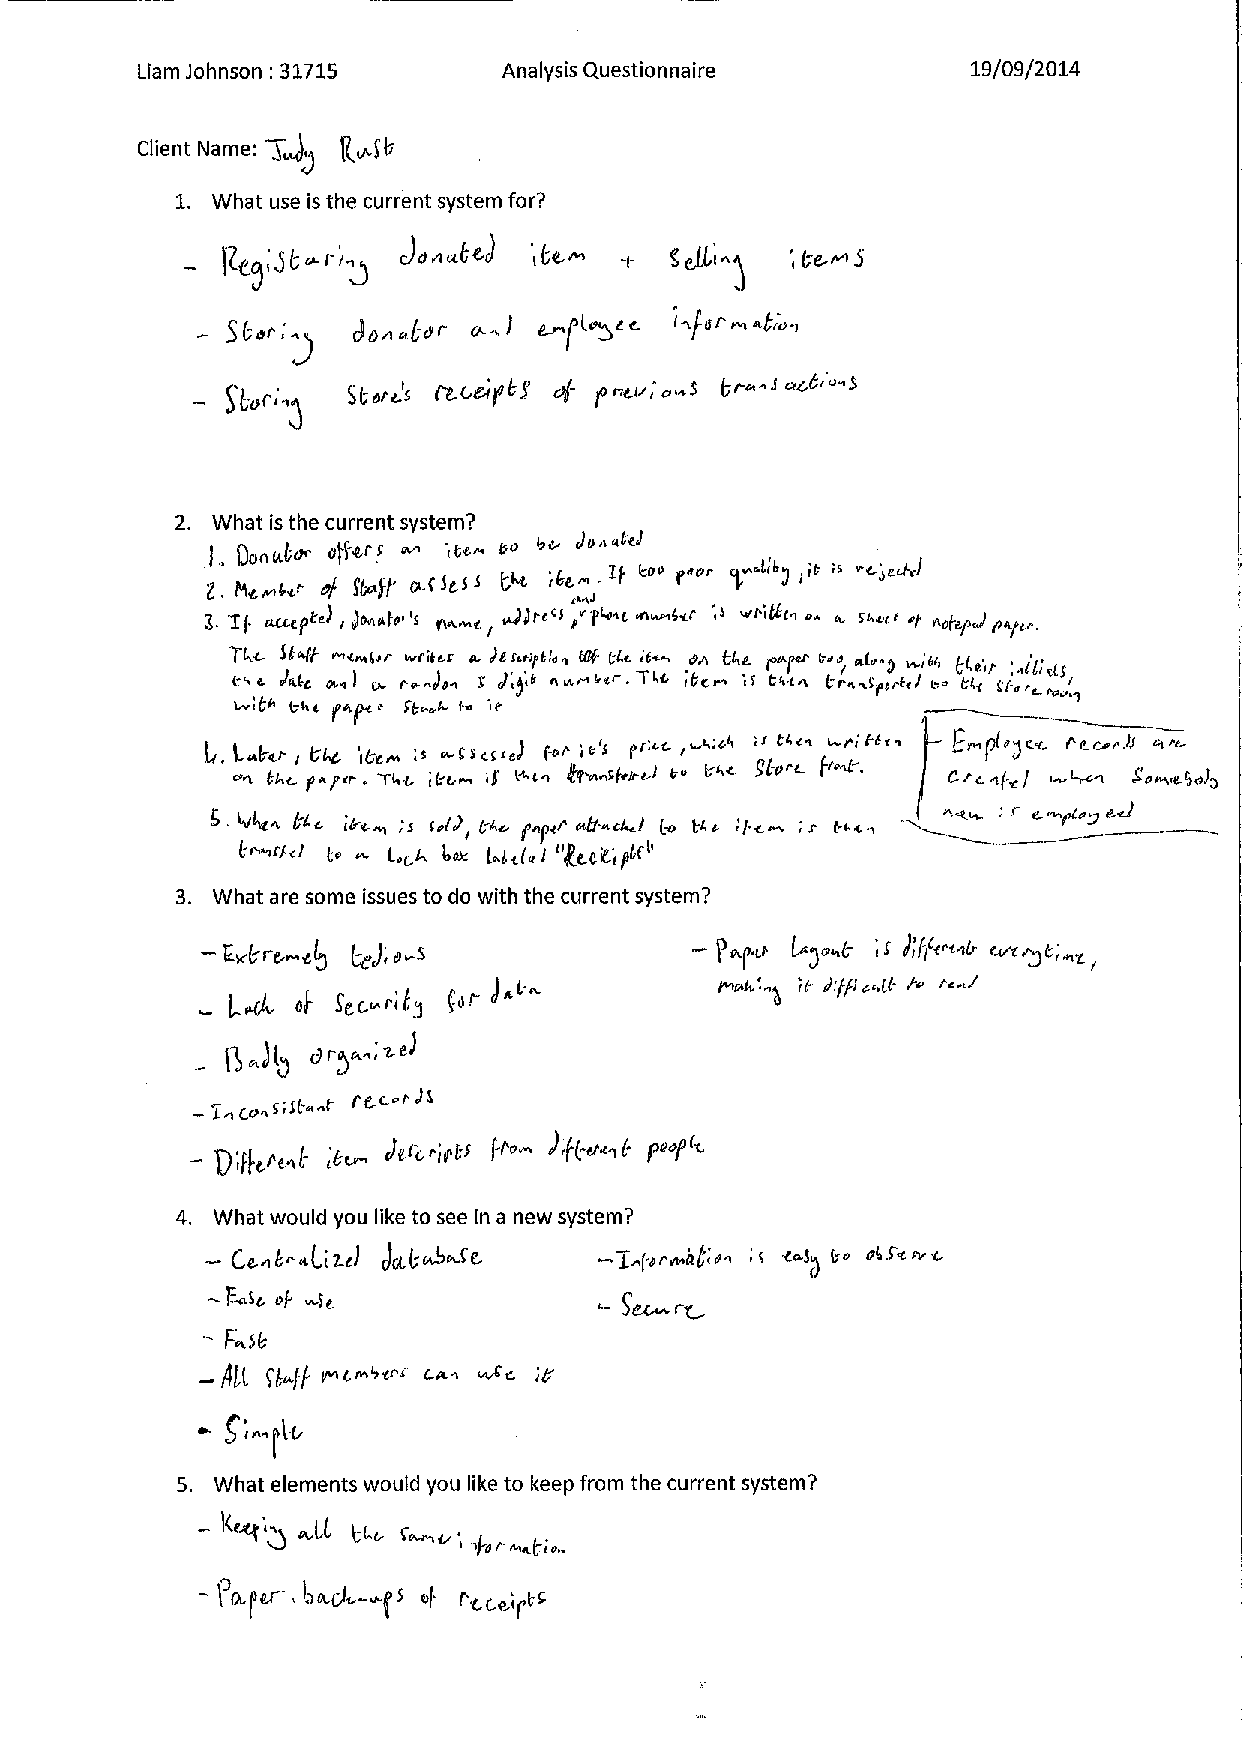
\includegraphics[width=\textwidth]{./AnalysisPDFs/SectionAppendix.pdf}
    \label{fig:SectionAppendix}
\end{figure}

\section{Investigation}

\subsection{The current system}

\subsubsection{Data sources and destinations}
The system that’s in place now uses these data sources: staff member, donator, and the item tag.
 Staff members information is currently kept in a paper based form in the private office of the shop. The data is stored on many different pieces of paper and each staff member has a paper folder with all of their own information in it. This information has the details of their name, home address, postal code and contact number(s). The details for their payment are more organized and are secured in a metal filing cabinet with a lock. This cabinet is not large enough to contain the employee information and their payment details. As mentioned before, a donator will leave their information with the member of staff, and these details get attached to the item before sale, and then removed and (badly) secured after sale.

    \begin{tabular}{|p{3cm}|p{4cm}|p{4cm}|p{2cm}|}
        \hline
        \textbf{Data Source} & \textbf{Attributes} & \textbf{Example} & \textbf{Destination}\\ \hline 
        \textbf{Staff Member} & \textbf{Initials, Donation Code, Item Description, Item Price} & \textbf{JJ, 71723, “A fridge”, £4.99} & \textbf{Item Tag}\\ \hline 
        \textbf{Donator} & \textbf{Name, Address, Contact Number(s), Item(s) of Donation} & \textbf{Johny Johnson, 7 Rinnocks Close, Herts, SY5 9CX, 0700502340, A vase and a flower} & \textbf{Item Tag/Receipt Box}\\ \hline
        \textbf{Staff Member} & \textbf{Name, Address, Contact Number(s)} & \textbf{Jamie Jameson, 8 Rinnocks Close, Herts, SYS 9CX, 01189991221; 09283745902} & \textbf{Employee Files}\\ \hline
        \textbf{Staff Member} & \textbf{Donator : [ Name, Address, Contact Number(s), Item(s) of Donation] Staff Member : [Initials, Donation Code, Item Description, Item Price] } & \textbf{[Johny Johnson, 7 Rinnocks Close, Herts, SY5 9CX, 0700502340, A vase and a flower], [JJ, 71723, “A fridge”, £4.99]} & \textbf{Receipt Files6}\\ \hline 
    \end{tabular}

\subsubsection{Algorithms}
The algorithm used in the process  of donation are fairly simple and often tedious, as it must be repeated every time a new item is brought in.


\begin{algorithm}[H]
    \caption{Check if the item can be donated}
\begin{algorithmic}[1]
\If{$"donated\_item.quality" <"minimum\_donation\_quality"$}
\Function{Refuse}{donated\_item}\EndFunction
\Else
\State $item\_tag.donator\_info \gets  donator\_information$
\State $item\_tag.staff\_info \gets  staff\_information$
\EndIf
\end{algorithmic}
\end{algorithm}

\begin{algorithm}[H]
\label{fig:repeat_pseudo_example}
    \caption{Repeat Loop}
\begin{algorithmic}[1]
\SET{$total$}{$0$}
\State
\Repeat
    \SEND{$"Please\ enter\ a\ number\ (0 to finish)"$}
    \RECEIVE{$number$}
    \SET{$total$}{$total + number$}
\Until{$number = 0$}
\end{algorithmic}
\end{algorithm}

\subsubsection{Data flow diagram}

\subsubsection{Input Forms, Output Forms, Report Formats}

\subsection{The proposed system}

\subsubsection{Data sources and destinations}

\subsubsection{Data flow diagram}

\subsubsection{Data dictionary}

\subsubsection{Volumetrics}

\section{Objectives}

\subsection{General Objectives}

\subsection{Specific Objectives}

\subsection{Core Objectives}

\subsection{Other Objectives}

\section{ER Diagrams and Descriptions}

\subsection{ER Diagram}

\subsection{Entity Descriptions}

\section{Object Analysis}

\subsection{Object Listing}

\subsection{Relationship diagrams}

\subsection{Class definitions}

\section{Other Abstractions and Graphs}

\section{Constraints}

\subsection{Hardware}

\subsection{Software}

\subsection{Time}

\subsection{User Knowledge}

\subsection{Access restrictions}

\section{Limitations}

\subsection{Areas which will not be included in computerisation}

\subsection{Areas considered for future computerisation}

\section{Solutions}

\subsection{Alternative solutions}

\subsection{Justification of chosen solution}
